\hypertarget{crip-tic-of-vignettes}{%
\section[Crip-Tic of
vignettes]{\texorpdfstring{\protect\hypertarget{anchor}{}{}Crip-Tic of
vignettes}{Crip-Tic of vignettes}}\label{crip-tic-of-vignettes}}

In these sections I situate this research at the tables of my context as
a disabled researcher, collaborator and artist, coalescing these
different backgrounds to bring together where my research is oriented
from. Here I am channelling Alice Wong and her many interviews from the
\emph{Disability Visibility Project} (2017), grounding this work in the
misfitting and disorientations of being disabled. I do this through a
\emph{Crip-Tic of Vignettes}, playing on the tych scales, from diptych
to triptych to other compositions, and Cripping it to a tic (Maier et
al., 2020) to hold the contradictory scales, relations and recursive
experiences these times unfold through. Instead of a static or linear
scaling as norm the Crip-Tic makes room for these vignettes to be
positioned inside, beside and beyond each other, whilst also holding the
possibility of more and less crip times to be held in relation. The
Crip-Tic also aims to hold these crip times not in a primarily
analytical form, which could undermine or filter their stories towards a
particular point, but instead holds them as Crip times in all their
complexity, forming wiggle room in my thesis for them to be held in
relation and refracted through later findings.

This assemblage in this research draws out four tics of crip times to
orient around and within. Crip times at the academic table, where access
is desired but superficial, with little negotiation of or room made for
what working with critical access and crip studies entails. Crip times
within the computational table, reflecting on the standardised forms and
their gaps to fill, the limited choices and obfuscated agencies within
computing and the technical systems that we are conformed to by our
everyday relations to institutions. Crip times on the operating table,
where care as treatment is executed within institutions, and where the
medical model invalidates and cures society of the sick through
configurations of violence and neglect. After these sections I turn and
retreat to crip times at the crip table, the table of disability justice
and life affirmation, and one where I have experienced radical sets of
crip care and politics in action.

\hypertarget{the-research-table}{%
\subsection[The research
table]{\texorpdfstring{\protect\hypertarget{anchor}{}{}The research
table}{The research table}}\label{the-research-table}}

In this section I will talk about experiences of being a Crip in an
academic institution in the U.K., and practising within the norms of
these research institutes. There are many examples of this within Crip
texts, for instance, Margaret Price's \emph{Mad at School} (2011), but
my experiences and tics are contextually specific and form an embodied
foundation for this work, the conditions it emerges from and aims to
address. I trace the very queer lines of bumping into, running away
from, and figuring out what feel like more cozy boundaries in relation
to academic institutions. If I return to Ahmed's brief reflection on
repetitive strain injury (RSI), how do these paths, these desks and
inherited orientations of work determine us to be broken before we even
start? In exploring these examples, I aim to open up how academic
practices and imaginaries of futures do not imagine us there before we
even begin, and in response we need to make lots of Crip trouble so that
we can wiggle ourselves in.

Accessibility in institutional terms can prevent disabled researchers
from being present at the table. For example, at a major science and
technology studies conference in 2024, accessibility was reframed, in
practice, to mean early career researchers but not disabled people or
other intersections of marginalised international communities either.
This was enacted through the logic of cutting costs on hybrid access to
fund early career researchers. In cutting the hybrid accessibility to
the event, disabled people who find it hard to access in person could
not easily be in dialogue, but also those with limited access due to
geopolitics and border regimes could not be present either. This left
some panels with a fraction of their speakers, falling short of being
accessible to these broader intersections of un-imagined communities.
The conference also had an inclusive set of food tokens for the event,
but with my dietaries I could not make use of most of them so ended up
paying for my own food on top as well. These everyday examples of
inaccessibility in academic spaces and institutional norm build up to
larger, sometimes exhausting, patterns that make these spaces unlivable
for many.

From here, I want to attend in more depth to how academic institutions
reproduce what Kafer describes as Crip-less futures. Specifically, I am
going to discuss a project in which I wanted to imagine with Crip bodies
what a future might be. In this experience I realised that academic
institutions often can't feel this Crip stuff in their framings of
accessibility, as they keep it at the edge of their reach, with no
capacity of being intimate. I was told many times what accessibility is
by able bodied people in these institutes, prescribed roles I must
follow and spaces and times I must fit to, often with my frictions,
labours and issues being hidden from view or easily packaged and moved.
In this reflection I share where and how I have taken care of my
bodymind and this Crip stuff, in order to speak up to and reorient the
institution's deterministic ableist configurations of futures.

I applied for a residency with a major research facility, let's call
them X - Digital Future Institute (or X-DFI). In placing the X here I
retain partial anonymity, but also refer to SoLiXG's definition of
XG\footnote{"``XG'' is an industry term for anticipatory technological
  iteration that we in SoLiXG extend to capture the process of
  developing, expanding and maintaining digital infrastructures, always
  with an eye to the next generation. As the media scholar Wendy Chun
  points out, this process is never finished and constantly gestures
  towards the next update." - https://solixg.net/keywords/xg}, denoting
the infinite growth of digital institutions, infrstructures, and
imaginaries. In SoLiXG's case this is the power of big tech network and
cloud ``solutions'', and in mine the ever-prevailing ableist institutes
of digital futures that will never imagine or be able to hold Crips in
their ``infinite'' futures.

I originally applied to this residency with the concept of making a crip
infrastructure in the form of a server accompanied by a relaxation
space. I explained clearly in my application that it was an
infrastructure made by and for disabled people that also included a
chill space for disabled people to decompress and relax. I expressed
clearly my desire that the online space and IRL installation were for
crips to have a safe and calm space to collectively imagine what crip
futures and practices online might look like. They accepted the project,
I was relieved as I could get paid to do some of my own work, and relax
about financial stresses. In the first meeting they told me they were
chose me because they liked that it was Crip stuff.

I was appointed a ``mentor'' who I met up with briefly. We began to chat
about the project and work, I discussed for minimum five minutes ideas
of creating infrastructures through non-prescriptive methods. He told me
he was the method man, he loved methods and it would be great if I could
generalise these methods. I didn't feel heard. I carried on talking
about network infrastructures, about alternative imaginaries of care
around their limits, from a Crip interdependent approach. He said he
didn't understand.

In the meetings following, the mentor repeatedly questioned the validity
of the project and my ability and capacity to make it, instead of caring
for its growth. He asked whether a relaxation space was a valid artwork.
I tell him there have been many works, by crip artists and others, such
as Carmen Papalia's \emph{Pain Pals}\footnote{https://leonardo.info/Criptech/eaat/pain-pals},
Navild Acosta and Sosa's \emph{Black Power Naps}\footnote{https://www.moma.org/magazine/articles/842}
and M.E.L.T.'s \emph{Rest Assured}\footnote{https://www.sonicacts.com/archive/rest-assured}
that orient this approach. Each of them talk about different groups
needing space to stop from the incessant efficiencies of late
capitalism, to sit in and make their own times and to feel safe. It
still didn't seem to be valid to him. He again questioned my capacity to
make the digital infrastructure, whether I was able to do what I knew I
could do (and had done before). Over email, they asked for quantities: ,
how long the work would be up, how much community I expected? Repeatedly
I had to explain what it was, how I was going to make it. Every time, he
exclaimed he didn't understand the theory or the practice, and asked for
validity again. There was no trust or affirmation of this Crip
infrastructure.

Initially my ``mentor'' told me verbally that the fee was just for me as
payment, and they would cover materials and expenses. I was already
putting more work into this infrastructure than the fee entailed, as I
cared for this stuff. When it came time to get materials, I sent through
expenses, and waited. This was during the period where the validity was
being doubted (which was realistically the whole time). I had to send
through renders to visualise to them what it might be, and costings of
materials which took more care and more time. I waited. I emailed to
follow up. I waited. The time of the project stood still, Crip
infrastructure frozen in-validity. They replied. The cost of the
materials now had to come from my fee, unless they were of value and
could be used by the X-DFI in the institution's futures. I told them
that this was not okay. A while later they offered a small sum, but I
still had to pay the majority for the proposed work. This dialogue froze
the project for at least a month, as I could not start until I had the
small amount of stuff I needed to care for the work. The fee itself then
also got frozen so I had to pay out of my pocket to get going. Due to
``institutional'' delays the payment time had become indefinite,
postponed to an unknown date. Due to these delays, I had even less time
to care for this stuff.

They delayed the submission a bit, but the damage was already done. I
did not really trust, through their actions, that this was a place that
could hold Crips, or imagined them being here in this X - Digital Future
Institute. There was no flexibility in this hard institute for Crips
there. The mentorship could not flex to understand, acknowledge or
listen to Crip methods, practices and knowledges, and instead turned me
into the problem that needed to be cured. Instead of making space for
and affirming these imaginaries, however haphazard they might have
seemed, they chose to judge it repeatedly, not finding it valid in their
terms. Their terms seemed to infantilize what they thought Crips had
capacity for, repeatedly asking me to just make something soft for
stimming, easily packaged and handled for when they present it to
conferences. They didn't want to handle an awkward Crip body or
infrastructure. The change of terms to finances also reduced my trust
greatly, as it showed they did not understand or legitimise financial
accessibility as a barrier, and that their word was not stable. Due to
the payment delays, funding changes and my financial precarity I had to
take on another job at the same time, developing an app for another
research project. This change of terms, and the eddies that flowed in
its trail are additive to the stress and relations that caused my last
flare up, and why I ended up back on the operating table I mention in
the next section.

After these initial fallouts, I just kept myself to myself and made the
infrastructure on the cheap. Though I in many ways had lost faith in
this residency, I carried on mainly for the funding and to make my this
crip infrastructure ``against all odds''. So I decided to approah the
work as a prototype of what Crip infrastructures might feel like. Using
the technical setup I had already knew and developed, but leaving the
community out of it whilst the X-DFI voices were still involved. I
accompanied this with some cute stickers I rendered and wrote their Alt
texts as Crip imaginaries of caring with and for digital network
infrastructures. I go on to talk about this infrastructure more in the A
Cozier Configure-ability chapter, but in this relation and on top of all
the other things I had going on I didn't have the capacity to get them
to listen to the nuances of this change or its reasons, so I just didn't
communicate it with them.

The first payment came through as we were getting ready to display,
months late. The accessibility of the space had been miscommunicated,
stating there was a lift, then there wasn't one, and then there was,
which made me anxious about showing there. It turned out it was fine. In
preparation for the show, they began quantifying again, asking questions
like, what's the maximum time for a person to relax in the space? They
didn't seem to feel time slots undermined crip relaxation or politics.
They repeatedly tried to put the work in a small single occupancy tipi,
to shade disabled people from the light, and maybe hide us away? It also
seemed culturally inappropriate to display my work in, as a white
British artist.

When it came to the time to show the work, even though we had been
promised all along that this would be open to the public, and my
application explicitly said the work was for the disabled community,
they had not listened and it turned out it was just for a private event
for the investors of this new building. It was for an event so private
that even we the artists were not invited to it. They used this
exhibition as the signing off of the works, and again used it to
pressure me into buying my own train tickets and paying for my own
expenses to set up the work. By this point, I couldn't be bothered to
argue against this.

I pitched up to the X-DFI, and was the first one there. I had a nice
chat with the receptionist and he offered me a cozy cup of tea. I waited
next to a wall of tech company logos. They turned up. We had a tour of
the X-DFI, with its brand new facilities in digital twin technology,
still half built, with cables and tubes hanging down. It looked
expensive, the jewel in the crown of this digital future. I told them it
was a dual use technology. They asked what that was. I told them it
meant it was made specifically to have both military and commercial
uses. They looked surprised. We went upstairs to the open loft space.
They had snacks that I couldn't really eat. Luckily, I always bring my
own.

I started to set up the work, I chose a nice side with good plugs and
ports. I got the server connected fine, and the site was up. I pulled
out the soft cushy cloud pillows I had made with a collaborator. They
looked surprised I had stuff. I placed the easy read, take home text of
the cozy intentions on the table. It was installed, it was a very easy
setup.

Soon after though, they came with stuff. Stuff they wanted to stuff in.
I hadn't been told about or consented to this stuff. They brought a
weighted blanket, which was nice, but was definitely prescribed, and was
for the institution and not for the Cozy-Cloud. Play-dough and colouring
in bits, that didn't really fit in and seemed to infantilize disabled
people. All of this stuff brought and placed in the space without real
dialogue or care. They stepped back, and asked again how accessible the
space really is, it seems a little technical for "disabled" people and
for people from the ``street''. I told them to access the work you just
have to try and relax. They didn't. I asked them who the people
categorised and figured to be from the street were? I explained I was
creating social access to technical practices and processes which in
some places of course will be a little technical, but I am trying to
make it as accessible as possible. He asked to edit the cozy intentions
of the server. I said no. He asked if he was not woke enough. I said I
don't think you have the right lived experience to edit a text by and
for disabled people. He eventually left me alone.

After they had taken their photo op, where I masked a smile, I left my
Crip centred space to be shown to the rich investors of this institute,
and we went for dinner. We went to a restaurant where they had tried to
make it accessible but it still wasn't great for me. I didn't want to
cause trouble again so just went anyway. We ate some dinner, I dared to
have one dish and we chatted. My ``mentor'' complained about how much
free work and excessive stuff he had to do to get anywhere in his career
and how much he felt he suffered. I thought he should value and care for
his time and capacity more. I chatted to other people around the table.
When we were finishing up, he got the whole table's attention and said,
``I really don't think artists suffer enough to make good work
anymore''. I stopped. I leaned forward, and I said, ``As someone who
lives with chronic pain, I really don't think any value should be placed
on suffering''. He suddenly and eventually went quiet. Later after
dinner he sent me a text to apologise, I am not sure if he realised what
these sedimented politics also meant for him, or if he had felt ``caught
out''.

I couldn't touch that Crip server for a while after this experience. All
of those intentions seemed sullied by this ``mentorship'' and exclusion
from the futures of X institutes. The longer term eddies, the subsequent
flare up, operations and appointments this experience and its stresses
had contributed to meant that trying to make a crip infrastructure for
and by crips for relaxation had in fact manifested itself into more crip
pain, stress and struggle when in relation to an X Digital future of
these institutions. Now, I am moving to care for these scars and tender,
frictious relations, to re-orient the spaces I have capacity in so I can
work within them cozily. In softer actions I have pulled out one of the
Cozy-Cloud cushions and now sleep with it, dreaming of X-C/CFI
(Crip/cozy future infrastructures) most nights. This experience is one
that has made me care even more for where I table my Crip stuff. Are
academic institutions able to, or do theyeven desire to hold this Crip
stuff? Or will their values, politics, relations and orientations always
hold it out of reach and disable them from caring for the stuff of Crip
futures?

\hypertarget{the-computing-table}{%
\subsection[The computing
table]{\texorpdfstring{\protect\hypertarget{anchor}{}{}The computing
table}{The computing table}}\label{the-computing-table}}

Here I am opening up the computing table and navigating to an inquiry of
the ex-cell (excel) table of institutional databases and the automation
of their administrative logics. I am approaching this through two
avenues here, though there are many other approaches I could take. The
first is to reflect on how I as an individual have systemically by
multiple institutions been placed and prescribed to specific cells
within tables by others as they translate my experience into evidence to
validate my care. Here I am thinking this through with Mia Mingus'
\emph{Forced Intimacy} (2017). I will also reflect on how I as a teacher
and carer for students have found the computational interface of access,
and the social relations of students' access needs often hidden or held
out of reach, making it harder to care for their access out of the norms
of these institutions.

The first step is opening the tab on how I have been categorised,
documented and (in)validated by both academic and care institutes.
Within both there has always been a separation between me and my
embodied knowing of my experience, and the computational cells that it
is put into. This separation is carried out by the ``expert'' or the
``specialist'' who ``knows'' what I am experiencing better than I do,
and who will translate and filter it into the abstract syntax and
figures that are valid within these political systems and institutional
relations. All of these orientations take what has happened to me, how I
feel about it and the sense I make from it, and de-legitimise and
invalidate them, to instead be stated in the abstract words and figures
they have sedimented out of reach of me. It is also with the understated
and normalised violence through which these invalidating logics are
instrumentalised. This has manifested for me as 9 years of my specialist
and carers denying my chronic pain, as ``studies and figures show that
part of my body doesn't have pain receptors''. This is until recently,
when another cell has been ticked even further out of my reach, and
certain medications for chronic pain have been legalised, and so
seemingly has my pain. It is also that another ``expert'' regulating my
workplace stress and need for access, and who was mediating the input
into its validating ex-cell table, was a manager who was additive to my
workplace stress. When I asked (as I had a number of times before) if he
could invite me to the relevant staff meetings for me, as I was part
time, his reasonable adjustment was instead to tell me to come to every
third one. In reflection this left me more anxious as I still wasn't
sure which to go to, or if I would get in the way. I also reflected to
myself here how meeting invites are a fairly standard practice, and the
computed table of the calendar event had space for this invitation, but
instead he just refused to action this.

Here, I approach the computing table through Mia Mingus' \emph{Forced
Intimacy} (2017). For her, this concept covers the many ways that people
with disabilities in need of direct physical care, can be forced into
intimate contact with those around them, who can often be strangers. She
also widens this scope to think similarly about how disabled people
often have to give up intimate information about ourselves to validate
our access needs, and yet often still don't have them met in return.
Little care is given to these relations within computing tables. When
working through getting my access needs recognised, and reasonable
adjustments made for my teaching role at my university, I had to go
through an assessment with an external equality diversity inclusion
(EDI) company for them to be validated. It being an externalised and
outsourced company was no surprise in the neo-liberal configuration of
institutions, but it did make me reflect on how desperate these bodies
are not to have disabled people within them. So much so that they have
others take care of us for them, others who can take the blame when
things go wrong, others who they can keep us from being intimate with,
and to stop us from being intimate with them, and others that they can
easily cut off when they do not have to follow EDI any more. In this
meeting, I spent 40 minutes with a person I had never met before, and
have never since. After I had validated my illness through telling them
among many such intimate things, including that I didn't drink as it
made me sick, they finished the meeting by tell me to ``not take
advantage of this access'' and for instance ``go out drinking, and call
in sick the next day''. I was astonished by the lack of care and
intimacy,, to not even pick up on this basic thing. I firmly reminded
them I didn't drink as it made me sick, and also used this place of
reaffirming dialogue to remind them that I was very sick, and their
report had real implications on my life, so please make it out as it is.
She seemed to listen, and the report was very firm and clear.

The fact is, often this intimate data is compiled only to lead to
inaction, producing what Ruha Benjamin calls the ``datafication of
injustice'' (2020, p.~117). This is evident when I reflect on the way
the institutions of care have computed me on their tables, and held me
in their cells. When being tabled in their systems, experts directed how
I was. This included GPs over the phone telling me they didn't think my
flare up and chronic pain was that urgent, so putting me on a longer
waiting list, saying if they changed anything I would still be waiting
just as long. This was until I spoke up, a cell was ticked and I was
seen in weeks. It also meant that I have to catch a bus or train for 1
hour each way to get my bloods done, as my ``specialist'' doesn't want
to do the ``homework'' that means the box will tick so I can get them
done by my local GP. Relevant information about my bodily experience and
care becomes lost in translation somehow. For example, I repeatedly told
medical practitioners about my bodily sensitivities and needs at three
points before I was operated on, yet at every point this was not
accounted for or recorded. When I asked my specialist at the time about
this, after the horrific fallout from this lack of intimacy, which I go
onto more in the operating table, he shrugged and said, ``of course''.
When I went back again after having passed out from a flashback, told
multiple people in A\&E I thought I had PTSD from my operation, none of
them cared or recorded it. When I next saw my specialist again, he
didn't know. In these experiences, I felt this sense that the only thing
that was being recorded about me was their observations of me,
specifically ones through mechanisms that gave ``exact figures''. How
fast was my heartbeat, what was my body mass index, what was the
molecular composition of my shit. My specialist summed up their
ideology:, ``You understand, as a coder, right? We need more data! Until
then, we can't know what is wrong with you''. In response to this I
wanted to explain how data is often an undermining factor of what is
evidence and who can make it, meaning myy needs were eternally delayed
or badly treated, as my embodied data and knowledge was not valid. I was
exhausted and coming to from being operated on violently so I couldn't
quite make this out to him, nor would he have been intimate with those
words. It is also part of this longer history, one where my documents,
figures and ex-cell tables from my last hospital had not been
transferred over, probably due to the repeated neglect I had experienced
there, but also maybe their desire to have this evidence of neglect
lost. Either way, this also contributed to me being placed violently on
the operating table without the care and intimacy I needed.

When I re-orient towards the computing table as someone who has to
navigate and access it as a teacher and carer within the academic
institution it helps to highlight how some of these dynamics come into
relation. To do this I will critique the web interface for the teacher
side of a student account, orienting the access of their access needs
through computed tables. The interface for the website as a whole is
very clunky and complex with many windows, tabs and sub menus to get
lost in. I have never been trained in this interface properly, nor has
anyone I know.. S4 is an appropriated commerce software that is similar
to ones I have encountered when working in retail jobs. No one had shown
me where the access needs of students were stored, even after I had done
the course on EDI. I asked my manager where they were so I could read up
on some of my students' needs. He didn't reply for a while and some of
the needs were somewhat urgent, so I asked again. He replied saying that
their access needs are confidential, so he couldn't email them to me,
but that they were in the interface somewhere, without giving me
direction. I eventually bumped into him in the office later that week,
and managed to get him to show me where they were. The student access
notes, as he showed me, were in a back tab of their student page. The
tab was called ``Related'' and the area the essential access information
was under was named ``Provisions''. None of this read ``access'' to me,
and all of it felt like a barrier. The information held here also felt
like it was quite static, and like it might be as equally hard for a
student to access and update their needs dynamically as it was for me to
find them, potentially leaving this information outdated. When I also
tried to link technician who were also responsible for these students
through to this access information on S4, they told me that they did not
have the permissions to access this information, so I would have to
share it with them manually for them to know. All of these social and
technical orientations place access and the information someone gives
about their own desires and needs around institutional care at the far
end of the table and well out of reach, especially out of touch of the
possibilities of intimacy and care for their access needs.

When I return to S4 to see what it does emphasise in place of access, it
is endless figures and values that regulate the student's progress,
mainly orienting attendance. As visualised below
(fig.~\protect\hyperlink{fig:360}{1}), from the university S4 basic PDF
guide, there is no space in this 360° student account to hold their
access or needs. Instead, when we examine their page there are constant
figures on the right, no matter what tab you are on, showing student
attendance in both doughnut and line graphs. Even when you are reading
their access needs you are still prompted by these figures, and how much
a student has been present or not. This is not the only place, as 95\%
of the interface on their profile and the information around them is
also different aspects of their attendance record, but all through
filtered gates presented by the teacher, expert and policy maker. This
ranged from check in codes that are easily shared to show presence,
marks from projects, and approval/denial of applications for things like
extenuating circumstances. Again like my own experiences of being
computationally tabled in care institutes, these are abstracted figures,
taken by others, or configured through datafied logics, denying
students' capacities to figure themselves out in relation to their own
education and institutional care.

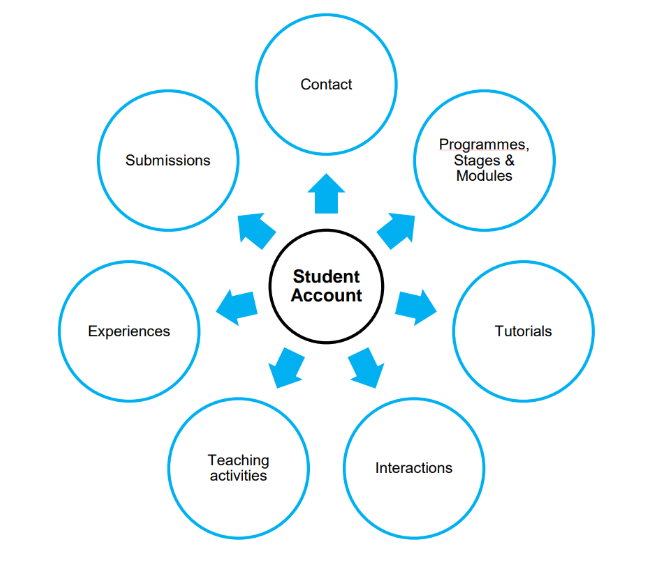
\includegraphics[width=9.23611in,height=7.90278in]{./media_02_Crip-Tic_of_Vignettes/Pictures/0.png}

Figure~1: Figure~1: S4 student account visualisation.

I share these frictions to offer up how these computed and automated
tables filter and put out of reach people with disabilities, their
access knowledges and their agency. It is, as I will go on to say more
in the Configure-able Methods chapter, not so much that these tables
cannot hold access, but that the experts, specialists and politics that
hold these relations in place keep access knowledges, disabilities
frictions and their radical criptiques out of reach. Access could be
displayed on the student account where the other figures of attendance
are, permanent, unavoidable and central to our relation and dialogue
with them, but instead it is squeezed frictiously and misfitting into a
pre-figured slot in a back tab of a sales software. In my own
experiences of being operated on and treated through the computational
tables a care institute, there was similarly no clear and effective way
for me to communicate my access needs within these ex-cells, as this was
configured as ``homework'' by an expect, instead of central to my care
and affirmation. This research orients away from this configuration of
computed ex-cells that hold, invalidate and hide disability, to instead
move towards social and technical practice and relations for these
systems that can affirm lives and centre these crip capacities for
radical access and care around computing tables.

\hypertarget{the-operating-table}{%
\subsection[The operating
table]{\texorpdfstring{\protect\hypertarget{anchor}{}{}The operating
table}{The operating table}}\label{the-operating-table}}

{[}!note{]} Trigger warnings of operations and medical pain etc. Skip to
The Crip table if you want to avoid potential triggers.

In this section, I will reflect on how the efficiencies of care
institutes and health systems leave Crip people on edge waiting for
minimal care at any unknown (or unknowable) point. Specifically in my
context of the UK National Health Service (NHS), as well as other
benefit and care systems that have been heavily underfunded through
``austerity'' politics we can turn to the work of China Mills (2018;
Mills \& Pring, 2024) to see how the health system has a direct effect
on the mental wellbeing and possibility of disabled life under these
violent times, policies and politics. Here I will bring into focus my
own embodied experiences of these relations, and how they made sense to
me as a crip researcher.

Here, I could talk for ages about the subtleties and changes in how my
injected medicine is scheduled for delivery around the hard efficiencies
of the system and not my capacities. Similarly I could turn to how Laura
Forlano rubs up against and hacks her medical devices and relations
(2023; 2016). I could discuss how I am a cyborg modified with biologics,
and connected to a refrigerated delivery pipeline. How this has slowly
changed without my input from a relation where the default was a call
from a caring person, who would help to guide and talk through the
process of arranging your delivery through to the current efficient
appified model, that pings, pokes and ``reminds'' you to go through some
fiddly forms, which you may not be in a good place to respond to. These
sets of relations are complex and situated though, and some people may
find this sort of automation frees them up to have more agency over
their care, whereas others may find this system cannot care for their
needs as it is too generalised.

What I want to rub up against here is the neo-liberal catchy rhetoric
around ethical automation. I heard the likes of ``a human in the
system'' at a UKRI \emph{social science conferences}, and which through
a few words aims to cure the inabilities of automated systems to care.
The irony is that there is always ``a person'' within a system if not
many, some trying to approach it, some developing and orienting it, as
well as the many maintaining it, but all of these positions and more
seem to be ignored. By their definition they aim to cure the inabilities
of the system by throwing another person in the middle, and this
generalised five word slogan cannot specify where they are or what they
are doing. You could throw in 100 more people, but if we do not care
about how, where or what stuff they are doing, we could be doing them
and the people, things and relations they are trying to ``care for'' as
much damage as if they were not there. This next section gives a more
precise encounter of automation without affirmation that I experienced
in my chronic care. The lack of intimacy in this encounter highlights
why the work of imagining and orienting towards affirmative
infrastructure is so essential.

In this section I will recount a recent experience of institutionalised
``care'' that left me with more violent damage to my body than it
benefited my well-being. This began when I had my third major flare up
of my life. This resulted mainly from being a crip person forced to work
over full-time to financially survive when I only have the ability to
work part-time. This relational fallout was due to unstable terms,
non-existent support networks, both institutional and familial, and the
invalidating exhaustive expectations of normative social roles. I have
already touched on these causalities and eddies in earlier sections, so
here I will orienting more around how in the aftermath of these
relations, and when in search of care, it became a struggle to have my
needs acknowledge let alone cared for. This reflection is also not meant
as a individual tale of a singular crip's treatment, but a place to
expand and fabulate from, especially in the UK. It is where I make room
and time for us to imagine the industrial scales that the
political/relations of institutional care tables operate through.

When trying to reach out for help it first has to be noted that I was in
the cracks of a system. I was between hospitals, not only due to having
moved locations, but also due to me running away from similar
mistreatment in my prior specialist department. This left me between
pipelines of care and treading water to stay afloat as I flared up with
no support beyond taking sick leave and time off of one of my four jobs
I had at that time. When reaching out for a referral to my local
hospital in Plymouth, both my GP and my previous carers both pointed the
finger at each other to initiate this change. After a while I pushed the
GP to initiate this move as I did want to get in touch or engage with my
old department. They put me through as a standard referral, even though
I was badly flared. After a month or two of ``self care'' I finally
received a referral letter with no date on it, but telling me to check
my contact details, ready for when they would contact me and a date
would be given. I decided this was not good enough and pushed the GP to
increase my urgency on the referral. In response he said that this was
unlikely to do anything and tried to convince me not to do it. In
response to this I told him that I was very much living in a reality
where these things felt unlikely to change and I just needed him to try
and see what would happen. After this strong defending of my needs he
agreed to raise the importance of the referral. ``Against all the odds''
this resulted in me getting a call to book in an appointment one week
later with my new specialist. In the virtual call with this specialist,
he very calmly tried to quell my anxieties by offering me multiple
examinations, from a low intrusive MRI, through to an intrusive
colonoscopy, both to find out what the ``problem'' is. At the time this
did comfort me somewhat but it became obvious that these were just words
and none of the care would be non-intrusive.

After this meeting I waited a few weeks, and eventually a letter came
through the post of another non-dated referral for a colonoscopy. This
time though it came with an enema kit, labelled, ``cleen, ready-to-use''
(fig.~\protect\hyperlink{fig:cleen}{2}). When I opened it up, I wondered
how long, if ever, it would take for me to be given an appointment. The
only thing I knew was that when the call came I had to empty my bowls
ready for them to violate my body to acquire the data that would
validate my pain, and the needs that I had already informed them of
verbally.


\includegraphics[width=11.11111in,height=11.11111in]{./media_02_Crip-Tic_of_Vignettes/Pictures/1.png}

Figure~2: Figure~2: Cleen and ready-to-use enema kit.

A few weeks later, somewhat fortunately, and somewhat stressfully, I
received another letter and call from the appointments team informing me
that I had been given a slot in just under two weeks' time. Time shifted
from an eternity into immediacy, taking me off balance as I was not
prepared to experience the same treatment that had left me traumatised
years before. The department's preparation for this appointment was
again a virtual telephone appointment with a nurse to do the
pre-assessment. In this call I tried to vouch for the type of care that
I wanted, asking to be sedated as I knew this was a painful experience
for me, and expressing that I had been previous difficulties with this
procedure. In response the nurse only played down my fears and told me
that it would not be as bad as I thought, and encouraged me not to be
sedated for the procedure, and just to take gas and air to alleviate
minor pain. I still tried to vouch for myself but ended up in a middle
ground of trying gas and air, to then turn to sedation if I felt it was
too much during the procedure. The thing I find extraordinary, beyond
the playing down of my fears, is that when I expressed previous
traumatic experiences in this area, they did not think to provide extra
care for this, in the forms of providing sedation, nor mental health
support going into it. They also did not ask for more information around
what happened and how to care for it. Fortunately, I have the capacity
to afford a private therapist that I have been seeing for a while and
they squeezed me in last minute, and coached me through the upcoming
treatment. It would have been very hard without this extra time and
care. These extra times though were too much for the institutions of
care to afford, and realistically had always been since the start of my
disability 7 years prior. This denial of more time to care when we table
sensitive bodies and relations in time is a denial and invalidation of
the affirmative types of care that these institutions and their
efficient capital configurations could hold if configured otherwise.

When it came to the day of the procedure, I was lucky enough to have a
support network that meant that it was possible for me to be sedated if
I needed to be. If I was isolated, like many disabled people are, and
without this support system of people to look after me for twenty four
hours after the procedure, I would have had to forfeit sedation, as
again the institution would not have the time to hold me. As I went in
with my friend, we were early to be checked in, so hanging around
awkwardly in the corridors of the hospital. When we finally went in to
register me, I went to the desk of the department, where I was greeted
by, as I guessed by their voice and demeanour, the nurse with whom I had
had the phone pre-assessment. Again this interaction seemed to play down
my fears and experiences, and pushed me to be squeezed and misfitted
into the efficient configures slot of their normative care of gas and
air and not be sedated as I had repeatedly asked. After this I waited
with my friend, and after 30 minutes I was ushered into another
pre-assessment room, where I was quantified, by weight, height and blood
pressure, and then left to wait again but by myself.

After sitting there for what felt like an eternity, with many thoughts
running through my mind, and anxieties growing, I started to question
and think about how to again try and advocate for the type of care that
would affirm me here. I took small steps to test the waters and
capacitiy for wiggle room within what felt like a very hard system.
Initially I started by just asking to go to the toilet, which I had not
been told where or if I could use. After this small success I had
started to build up the momentum to feel like I was able to vouch for
the type of care that I really needed. I was eventually taken through to
the operating table, where I was briefly introduced to the two men
operating on me who I had never met before, nor had a virtual call with.
They went on to lay me down and prepare me for the operation, it's hard
to remember but it initially felt like my desires to be sedated had not
made it through. It was only when I stated the word ``traumatising'' in
relation to my prior experiences that his eyes lit up, and he started to
take me seriously. It is hard to say here whether that was in relation
to providing me with the appropriate care for my situation, or whether
it was that by stating these words I had gained leverage by holding him
accountable to his actions.

I still for some reason felt obliged to try and be shoehorned into the
efficient slot of non-sedation, and have the sedation as a backup,
something I will not do again. To prepare for this he went to put an IV
in my left arm. After having my blood taken many times, every three
months for the last 7 years, I am used to the pain and know what to
expect, and also get complimented on how easy my veins are to find. As
he slipped in, I felt more pain than normal, a sharp sting that I
flinched at; as he tried to draw blood it worsened and so did my
reaction. Disregarding my response and feelings and after a few more
painful attempts to get it to flow he pulled out, telling me that I had
not stayed in-line with his needle. I began to cry, feeling no trust in
this person, or in how they were about to operate on me. I lay there
still. Without a glance he moved to the other arm, and proceeded to try
again. This time I was internally trying to stay in-line as much as
possible as he slid inside of me. This time it felt the same as any
other, and this time I did not flinch.

This is also the time that I passed out, not that time at that table,
but the time just after writing the last paragraph at this table. Twenty
four hours later, writing this having again been treated by the NHS,
this time for passing out, for falling from a counter chair, and for
hitting my head on the ground. All because I dare to remember that time.
I think it's safe to say that I will not be writing about that time, but
I can tell you worlds collapsed, sedation through party drugs doubled by
bodily violation and immense pain brought memories, spaces and feelings
in-line and out of time. I blacked out from pain and I awoke still
crying.

Waking up on the floor after passing out remembering this, this time. I
was assisted by the staff of the coffee shop. They helped me sit up,
drink up and come to. They did, however, immediately get me to sign an
accident waiver form to make sure that they would be covered around this
individual ``problem''. They asked why it happened, I could not say. I
texted my friend, and she said she was on her way. When I was doing
better I gently walked home, around the corner, where she met me. I felt
obliged by norms of rational care to call up 111, the low emergency
support number in the UK. I felt okay, and had no clear signs of
concussion, but the rationale of their care insisted I go back to the
hospital, the same hospital I had remembered. They told me it was
urgent, so I should pay for a taxi, but not important enough to send an
ambulance, but they would be waiting and ready to receive me. I went in
again, they did not know who I was and were not ready for me, sitting
there like human livestock, watching people go mad around me in these
sick times. I was quantified, I had my vitals taken after a few hours,
but nothing said to me, just that it wouldn't be so bad. I waited
another few hours with nothing said to me. I finally asked what was
going on, they told me I had another 3-4 hours left to be seen. A senior
doctor, not in the conversation and with his back to me looked over his
shoulder said, ``you should probably go home''. I asked, ``do you know
why I am here?'' He did not, even though I had told four people why I
had passed out, because I had remembered. Their table of operations
could not hold this information. They told me ``that I had decided to
come here'', and so ``it was on me''. I told them ``111 had told me to
be there'', so I felt like I had to go here, if it was up to me, I would
have stayed home from the beginning. They didn't reply, I took a
complaints number and left. I still haven't complained because I am not
sure what it will do.

As I woke up after the last time, crying, in came the ``specialist'' who
had done this to me. He told me how my body was, he told me that I was
having fast movements, when they were actually very slow, and told me to
take medicine to slow me down further. I refused. He told me that I
wasn't so inflamed, I told him it had been months since I was, so was
starting to settle after my own care. He told me that when you focus on
sensing something too much it can start to hurt more than if you ignore
it. I had just stopped heavily dissociating from my body that year, and
focusing on my body and feelings was helping me to get stable. He tried
to get me to take more biological and immunosuppressant medicines as a
quick fix. I refused and vouched for the type of care that I wanted:
mental, dietary and financial. He looked confused. He then started to
prescribe me dietary advice whilst I was still reeling in pain and
confusion from this experience, not in a way where it was helpful, but
in a way where he reinforced his expertise and role as a ``specialist''.
He left, my friend picked me up, with another giving me a lift home.

On my own Crip timeline of writing this thesis, it took me a month just
to start writing again since being on the operating table, as I could
not find the words. No one in those institutions and from that time
called me up for aftercare. My bodymind was much worse off after being
treated by them and it has taken many more than months to heal it still.
These treatments, these performances of efficient industrial care and
this experience have still not benefited me in any way so far, just left
more scars on my bodymind. I again stepped out from this public
institution and into private care, in the form of paying for myself to
have a dietitian and try to improve things. This time, I think because I
had paid for it, I had someone's time and this time they listened and
cared. Over this time, I started to get better again.

The ``specialist'' who had done this to me, had, however listened
somewhat and gotten me a dietitian from the NHS. This appointment was
more disorienting than helpful though. Even though I had been making
progress, been gaining weight, been feeling better in my body, they told
me that I should stop what I was doing and have a normal diet. That I
should just be normal, otherwise I might be doing damage to my own
bodymind, and that the feelings and practices I had grown in relation to
my expertise where not okay. They didn't give me any advice on how to
become ``normal'', just that I should be, and that I should also start
eating things that I knew were painful to eat. They also told me I
should get on more medication as a quick fix, even though I am not sure
they were qualified to recommend this. Quite inappropriately they were
also the one to tell me the results that came back from my operation,
and that I was still inflamed, even though he had told me I wasn't when
I awoke. This was over a month later and no one had reached out to tell
me this before. They also told me I had a different condition to what I
had been diagnosed with before. I left disenfranchised, disoriented and
dissociating.

I later had another appointment with my ``specialist'' as a follow up a
month or two later than the dietitian. I arrived on time, the
appointment was delayed. I waited an hour and a half. He finally made
time for me. I went in, and he was already high energy, it was hard for
me to orient around this anxious energy. I asked if I could record the
meeting to listen back and chat about it with my sister. He said no and
started saying I was trying to post him online, and set him up, I was
not trying to do this. We ended up getting a nurse to help mediate the
conversation. It carried on with this type of dynamic for the entire
appointment, with him taking an hour to even ``remember'', acknowledge,
and validate what happened in my last operation by him. Continually
after this point he tried to make me feel bad for taking more time than
my appointment allocated, of needing too much, and trying to shake me
off this table. When we finally got past him acknowledging the operation
happened we finally turned to future care for me, where he still told me
I had a different condition to what I had been told all along. I
contested this, but he said he knew, even though he did not have the
files from my old hospital, as they had not been transferred. In a later
meeting with my specialist nurse, which was actually the first close to
affirmative appointment I had, she finally acknowledged that I had the
condition I knew I had, and proven through the data my ``specialist''
had misread. She also noted that some of the medication that he had
suggested would not have helped, was inappropriate and may have made
things worse. The thing I found profound, and which is a sedimented
critique of the medical model and pharma-capitol is his normalised move
to prescribe very expensive, high side effect, and restraining
medication, rather than provide social relational care for me. Instead
of listening from the beginning where I asked for a dietitian, a
therapist and some space to reorient my bodymind and which cost roughly
the same if not less that the medication he wanted to prescribe, this
``data'' was invalidated, to instead go on a deep and violent
exploration to the truth of the problem, which I already knew . . . was
in the system.

I don't recount this as a sympathy plea, as to say that I am the one
suffering, or to recourse revenge on the problematic people in these
systems, but to make room on this table for this stuff. Compared to
other disabled people under the current economic system, I am a
relatively financially stable person, and if you know me you know I am
also very able and willing to defend my boundaries. I am also white and
often perceived as a man by these institutions, which is frustrating,
but all these things will orient the type of care I receive. This is one
incident in my own life, and sits here as a frictious contour, a
misfitting of needs, and a cliff to look over the bodily horizon of
these institutions of care. It is to to make room to bring in the
background of disability the norms of the institutions invalidate and
ignore. Not as a matter of fact, but a fact that matters, and matters
more when we fabulate to hold the many stories of people within this
industrial grinding down of care. Ones which are much worse than this.
Sitting in the A\&E for 5 hours was enough to see these lives, these
times, and these bodyminds being driven mad and made sick in the
presence of institutional care. This institution is not meant to hold
all of these lives, experiences and pain, as it was never imagined to.
This recollection of the operating table is here to wedge open the door
from slamming shut and let these feelings spill through into dialogues
of affirmative infrastructures. How can these Crip experiences,
practices and wisdoms around institutions, around just refusal and
self-advocacy, be in relation to those that wish to operate on us? How
can they inform critiques of the current configurations of care and
imagine the times, spaces and futures we really need? When I say really
need, I mean really need.

\hypertarget{the-crip-table}{%
\subsection[The crip
table]{\texorpdfstring{\protect\hypertarget{anchor}{}{}The crip
table}{The crip table}}\label{the-crip-table}}

Here is in many ways where I start to turn away from these other tables
I have been institutionally forced to be in touch with and instead turn
to the crip table that this research orients towards. This turning
towards other crip tables is in many ways the retreat that I take
throughout this research, and this inquiry aims to offer up reasons and
sense making for why I have made room for the radically affirming crip
politics in action. To do this I reflect on the times I have been
inspired and my perspective shifted around what is not only possible,
but what we could be orienting towards collectively through disability
justice and collective access. This inquiry reflects on the simple ways
I experienced M.E.L.T. centre rest and relaxation in their \emph{Rest
Assured} workshop with Sonic Acts. It also reflects on the ways that I
felt guilty for the abundance of access and care that I experienced at
Healing Justice London (HJL), Transformational Governance Collective and
Beyond the Rules' seminar \emph{Life Affirming Organisational Practices}
(Dhami, 2023). These experiences have informed the capacities I desire
for the people around me, and myself when approaching the crip table.
Much of this research has been an effort to put these life affirming
relations I have been in touch with so briefly as the places I centre
and orient from. This practice aims to overflow with abundance in my
daily life and my organisational/institutional/infrastructural
relations. This also stems from me, through this research, finally
acknowledging my own disability, after 7 years, 3 flare ups, and many
disabling social relations. After all this time, it is the radical
relations this put into reach for me that made room for this work to
feel at once acknowledged, validated and cared for, instead of having
these practices, knowledges and labours backgrounded or hidden from
view.

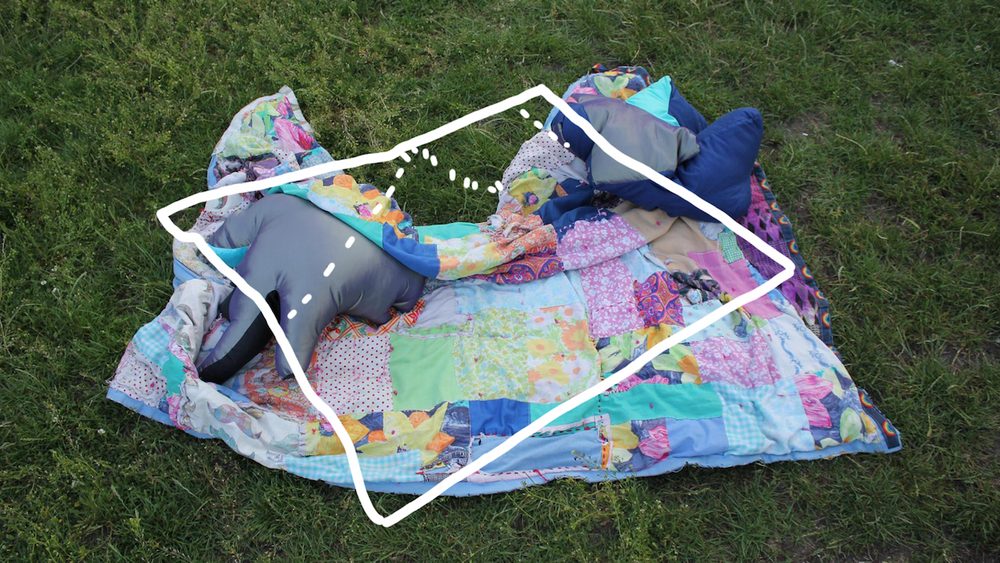
\includegraphics[width=13.88889in,height=7.81944in]{./media_02_Crip-Tic_of_Vignettes/Pictures/2.png}

Figure~3: Figure~3: Visual for Rest Assured by M.E.L.T.

M.E.L.T.'s \emph{Rest Assured} workshop was one of the first Crip
encounters I had in my research, and life (knowingly). This was held as
``an online reading group on non-normative ways of experiencing,
theorising, materialising, subverting and being in time''. This in
action felt like a reading group of Crips coming together in the most
tender and soft ways. Some of the things that touched me most were
within the actions of care and time M.E.L.T. took to make the space so
easily accessed by all members. This included things like access
copiesof the upcoming presented/spoken text, which enabled us to follow
along with the program and see what was coming ahead, so we could plan
our capacities ourselves. It was also through the affective ways we felt
in the space, how we were introduced to this reading group through a
meditative relaxed listening of Kevin Gotkin's \emph{Artist in
president} talk (Kevin Gotkin 2021). The way we were also prompted to
share mixtures of visual prompts and texts to represent how we felt, and
what sort of capacities we had at that time. This group was made up of
what they called 2.5 sessions. This was two full sessions, with more
than 0.5 of room made for asynchronous interactions and exchanges. I had
a mixture of things going on, from being tired, busy, anxious . . . I
only made it to the first one. You could say that this made me miss out
on knowing what happened within the workshop, but this specific very
Crip position also oriented me to be able to know how this workshop was
made knowable and flexible to these other temporalities and rhythms .
The access copies they provided made room for me to catch up in my own
time what had been going on within later sessions, and how they had
approached and oriented these texts. Alongside this, and in between, was
a shared Signal group chat where members shared excerpts of their lives
and times that related to reading themes, as well as where we were in
relation to them. Becoming in touch with these radical crip
possibilities and practices of bringing people together in and out of
sync, and through multiple points of contact, media, temporalities and
approach really re-scoped my imagination of what collaboration and
access could be practised as and made known through. It made me
reconsider how I could structure, order and configure my relations,
process and practices around a Crip time, interdependent care and
critical access.

Another key instance of coming into contact with radical Crip tables of
access was that of Healing Justice London (HJL), Transformational
Governance Collective and Beyond the Rules' day long seminar called
\emph{Life Affirming Organisational Practices}. These collectives held
many different workshops and talks throughout the day, again through a
combination of embodied practices, mixed media reflections, and
collective dialogues. For me, even though I was by myself (and awkward
and shy when so), this place was so welcoming, especially in comparison
to the academic conferences I had experiences of. One moment that
emphasised this to me was when I had booked a 1-2-1 with one of HJL's
admin team to get advice on organising with In-grid, a collective I'm
part of and inquire with later in this research. Even though they seemed
slightly confused as to who I was, what In-grid as an
organisation/collective did, and why I was talking to them, they still
took time and care to advise me on how to organise with In-grid through
radical care and life affirmation. Her feedback, and many of the
messages of the day were fairly clear, and focused on making power
known, and caring for the frictions and pains it holds, and in doing so
make it transferable and transformable. Here she recommended we, as a
very decentralised organisation, try to introduce a Raci matrix to map
roles and responsibility, as well as doing skills audits to help with
this. Through these practices, we can try to make accessible and
knowable the skills and power within our community, so that we can
collectively care for them, instead of individually controlling and
reinforcing unwanted relations of power. This feedback is still very
much in process within In-grid (as I think it will always be), but from
this care-full recommendation we have started at least to structure and
try to make room to figure out our flows of power in projects and make
accountable our relations within them.

The \emph{Life Affirming Organisational Practices} event also
transformed my scoping of the possibility and promise of access.
Compared to other academic institutional conferences I had participated
in, there was so much care, thought and abundance when it came to
access. This change in relations in many ways made me feel guilty for
having been offered these modes of access. Where normal institutional
conferences would charge a (large) fee, often not cover travel, and be
just in person, this event gave grants for travel, admission fee
waivers, and different modes of attending. Where academic conferences
regulate and validate their grants, this event was offered without any
need to validate your need of them. Unlike institutional systems I have
mentioned in the computing table that force intimacy, table you and
invalidate you, this group just gave if you asked, and trusted you.
Reflecting on this feeling of guilt, it made me ask why was I feeling
guilty here when I was finally having my needs met. I contemplated it
might be that I had not filled in any forms, so I was unsure if I was
valid or not, but dismissed this. I realised for me, in many ways it
aligns with a guilt proposed by Audre Lorde\footnote{``Guilt is not a
  response to anger; it is a response to one's own actions or lack of
  action. If it leads to change then it can be useful, since it is then
  no longer guilt but the beginning of knowledge.'' - (Lorde, 1997,
  p.~282)}, where it is a guilt of inaction, both from myself, but also
from those around me and from the institutions that hold these ableist
inaccessible relations in place. When in touch with such radical care,
access and affirmation it informs us not only what we have not been
doing or vouching for ourselves, but also as teachers, collaborators and
organisers, what we have not been doing for others. Moving on from this
feeling and sense making of guilt and into the joys of actioning its
sense I have been building up my own capacities for understanding,
navigating and caring for access in ways informed by being in touch and
at these care-full crip tables.

The final thing I want to touch upon at this table and that has informed
my approach to this research and collaborations, is some of the
practices and concepts shared in HJL's \emph{Why Somatics? Growing the
Embodied Capacity for Transformational Governance} workshop. During this
very embodied workshop, they surfaced an understanding and approach to
practising life affirming infrastructures and institutes, stating that
``broken people coming together will only ever make more broken
systems''. This does not reproducethe preconception that we can cure
these people or systems, but suggests that to move towards an affirming
one, we need to first heal ourselves, to then care for those around us
through these systems and infrastructures. It also helps me ask, how do
I ally? What do they need? Then, from this orientation, I can start to
care for the relations of these institutions, infrastructures and the
politics they want to configure.

\hypertarget{dancing-with-tables}{%
\subsection[Dancing with
tables]{\texorpdfstring{\protect\hypertarget{anchor}{}{}Dancing with
tables}{Dancing with tables}}\label{dancing-with-tables}}

This research in many ways orients a certain dance between these
separate, but overlapping institutional tables. In many ways this is
framed as a retreat in this work, of trying to put the violences of
certain tables out of reach, and orient them towards notions, politics
and practices of radical crip life affirmation. In this retreat though,
and through a Crip understanding of the cyborg, we are still attached to
and entangled with them. Through being in relation with these
institutional tables of computing, academia and care, I can also shape
them in return. It is this refusal to stay in line and to give feedback
where it is not wanted. It is when I come to the operating table and
finally talking back to the ``expertise'' of my ``specialist'', not only
to refuse medicine and advice that will harm me, but also asking if he
had ever read any disability studies? When he said no, I said, ``Don't
you think it is interesting you have never listened to the people you
care for?'' It is when I come to the computing table and the student
account interface and feel the normative urge to police them for their
attendance, to instead ask myself, ``How do I care for this person and
to be an ally in their building of capacities?'' It is now that I have
my own capacity to sit at research tables and send emails telling people
what my needs are, and defining good boundaries around them. It is me
writing this research and making wiggle room for these reflections and
inquiries that maybe give too much information, emotion and anger, but
offer within that the capacity to hold these necessary points and times
out of line so to disorient and manifest this work from.

In this dance I make many mistakes, I am clumsy, I am mad, I am Crip. In
this dance I take just a few steps, a couple back, a number sideways. In
this dance and between these tables, as I get to grips with them, as
they try to shake me off, and as I try to hold on, I build my capacity
to reorient them. The shaping effect that some have on me I also have on
others, and it is within these frictions, flows, rhythms and moves that
this research starts to manifest itself. Again, not through one point
but a repetitive Crip-Tic and recursive practice of wiggling room
within, between and around the capacities of these hard systems and
institutes for our communities and their many tables to be cozily in
relation.
